\documentclass{beamer}
\usepackage{xeCJK}
\usepackage{graphicx}
\usepackage{xcolor}
\usepackage{setspace}

% ============= setup =============
\setCJKmainfont{Taipei Sans TC Beta}
\setCJKsansfont{Taipei Sans TC Beta}
\hypersetup{
    colorlinks=true,
    linkcolor=black,
    urlcolor=blue
}
\renewcommand{\baselinestretch}{1.25}
\usetheme{Madrid}
\usecolortheme{crane}
\setbeamertemplate{items}[circle]
\setbeamertemplate{section in toc}{\inserttocsectionnumber.~\inserttocsection}
\AtBeginSection[]{
    \begin{frame}
        \vfill
        \centering
        \begin{beamercolorbox}[sep=8pt,center,shadow=true,rounded=true]{title}
            \usebeamerfont{title}\insertsectionhead\par%
        \end{beamercolorbox}
        \vfill
    \end{frame}
}

\title{實做能力加強}
\author{temmie}
\date{}
% ============= setup =============

\begin{document}

\begin{frame}
    \titlepage
\end{frame}

\begin{frame}
    \tableofcontents
\end{frame}

\section{位元運算}

\begin{frame}
    \frametitle{為什麼要學這個?}
    \begin{itemize}
        \item 因為電腦的機制,位元運算會比一般運算更快一些
        \item 在\textbf{枚舉}這堂課上,我們會用到很多
    \end{itemize}
\end{frame}

\begin{frame}
    \frametitle{進位制}
    \begin{itemize}
        \item n 進位代表只用 n 以內的數字組成(如果超過 10 就用英文)
        \item 二進位的數字代表只用 0 和 1 組成
        \item<2-> 如果一個式子有不同進位制的數字,則會用括弧備註在右下角
        \item<2-> 例如:$17_{(10)}=10001_{(2)}$
    \end{itemize}
\end{frame}

\begin{frame}
    \frametitle{二進位轉十進位}
    \begin{itemize}
        \item 以 $10001_{(2)}$ 舉例
        \item 我們可以先把所有 2 的冪次列出來:$2^4$、$2^3$、$2^2$、$2^1$、$2^0$
        \item<2-> 和原本的二進位字串一一對應後相乘
        $1\times 2^4$、$0\times 2^3$、$0\times 2^2$、$0\times 2^1$、$1\times 2^0$
        \item<3-> 將所有數字相加
        $1\times 2^4+0\times 2^3+0\times 2^2+0\times 2^1+1\times 2^0=17$
    \end{itemize}
\end{frame}

\begin{frame}
    \frametitle{十進位轉二進位}
    \begin{itemize}
        \item 詳細作法如下圖
        \item 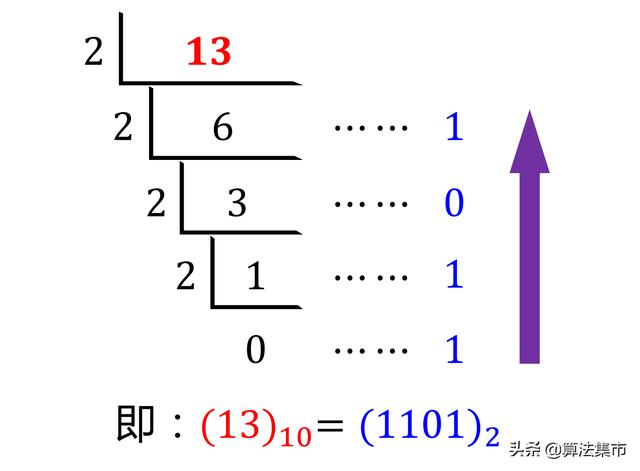
\includegraphics[width=7.0cm]{img/img_1.png}
    \end{itemize}
\end{frame}

\begin{frame}
    \frametitle{例題}
    \begin{block}{二進位制轉換}
        \href{https://zerojudge.tw/ShowProblem?problemid=a034}{題目連結}

        給你一個十進位的正整數 $n$,輸出 $n$ 的二進位
    \end{block}
\end{frame}

\begin{frame}
    \frametitle{位元運算的類別}
    \begin{itemize}
        \item 主要有 OR、AND、XOR、NOT
        \item 和一般的 or、and、not 不同的是,可以對數字做運算,而不是限制在布林
        \vspace{0.5cm}
        \item<2-> $AND$: 「 & 」 表示,如果兩個 bit \textbf{都是} 1 就是 1,否則為 0
        \item<2-> $OR$: 「 | 」 表示,如果兩個 bit \textbf{至少}有一個 1 就是 1,否則為 0
        \item<2-> $XOR$: 「 ^ 」 表示,如果兩個 bit \textbf{恰有}一個為 1,否則為 0
        \item<2-> $NOT$: 「 ~ 」表示,將 1 變成 0,0 變成 1
        % 記得手算真值表舉例
    \end{itemize}
\end{frame}

\begin{frame}
    \frametitle{使用位元運算}
    \begin{itemize}
        \item 難道用位元運算還要手動轉進位制? @@
        \item<2-> 在 C++ 中,直接對兩個十進位的數字做就可以了
        \item<2-> $17_{(10)} \mid 5_{(10)} = 10001_{(2)} \mid 00101_{(2)} = 10101_{(2)} = 21_{(10)}$
    \end{itemize}
\end{frame}

\begin{frame}
    \frametitle{例題}
    \begin{block}{位元運算的大雜燴}
        \href{https://codeforces.com/group/S6XjkGb6qB/contest/403070/problem/B}{題目連結}

        給你三個參數 $x$、$y$、$z$ ,找到 $(x \oplus (y \mid z)) \oplus (x+y)$ 的最小值

        其中 $\oplus$ 是 XOR 的意思,$\mid$ 是 OR 的意思
    \end{block}
    \begin{itemize}
        \item<2-> 參數數量是固定的,那就列出所有情況吧!
        \item<2-> 把六種組合各試一遍就可以了
    \end{itemize}
\end{frame}

\begin{frame}
    \frametitle{更多位元運算}
    \begin{itemize}
        \item 另外常用的位元運算有左移和右移
        \vspace{0.5cm}
        \item<2-> 左移: 「 << 」 表示,代表將所有 bit 左移 n 位
        \item<2-> 右移: 「 >> 」 表示,代表將所有 bit 右移 n 位
        \vspace{0.5cm}
        \item<3-> 例如: $17_{(10)} << 1 = 10001_{(2)} << 1 = 100010_{(2)} = 34_{(10)}$
        \item<3->你知道嗎?實際上左移就是乘上 $2^n$(右移則相反)
    \end{itemize}
\end{frame}

\section{字元轉換}

\begin{frame}
    \frametitle{ascii}
    \begin{itemize}
        \item 我們都知道電腦是儲存 0 跟 1,並不能儲存字元
        \item 那要怎麼儲存字元呢?
        \item<2-> 只要把所有字母編碼就可以啦!
        \item<2-> 實際上我們用的字元都有一個編碼,稱為 ascii 編碼
    \end{itemize}
\end{frame}

\begin{frame}
    \frametitle{ascii}
    \begin{itemize}
        \item $[\ 0-9\ ]$ = 48 $\sim$ 57
        \item $[\ A-Z\ ]$ = 65 $\sim$ 90
        \item $[\ a-z\ ]$ = 97 $\sim$ 122
        \item 利用編碼的連續性,就有很多功能可以應用
    \end{itemize}
\end{frame}

\begin{frame}
    \frametitle{例題}
    \begin{block}{數字總和}
        \href{https://codeforces.com/group/S6XjkGb6qB/contest/403070/problem/C}{題目連結}

        你有一個數字 $n$,請你求出所有位數的總和,保證 $n$ 的位數 $\leq 10^5$
    \end{block}
    \begin{itemize}
        \item<2-> 字串很大,看起來沒辦法用 int 儲存,所以只能用 string 儲存
        \item<2-> 我們可以用 for 得到每個字元,並且\textbf{減去 '0'},就可以轉換成數字
        \item<2-> '0'(48)-'0'(48)=0,'1'(49)-'0'(48)=1
        \item<2-> '5'(53)-'0'(48)=5,'9'(57)-'0'(48)=9
    \end{itemize}
\end{frame}

\begin{frame}
    \frametitle{例題}
    \begin{block}{凱撒密碼}
        \href{https://zerojudge.tw/ShowProblem?problemid=b516}{題目連結}
        
        給你一個字串 $s$,把每個字母向後移 3 位,例如 A → D,Z → C
    \end{block}
    \begin{itemize}
        \item<2-> 我們可以將每個字母的值都加上 3
        \item<2-> 如果該字母超過 'Z' 的話就減去 26
    \end{itemize}
\end{frame}


\section{陣列的使用}

\section{區間問題}

\end{document}